\documentclass[../TST.tex]{subfiles}
\begin{document}
\begin{pproblem}
A ball of mass $M$ has velocity $v_0$. It strikes a ball of mass $m$ ($M>m$) at rest. The collision is elastic. The angle between the velocity vectors of $M$ before and after the collision is $\alpha$.
\begin{subpart}
\item Find the maximum value of $\alpha$.
\item Find the velocities $u_M$ and $u_m$ of the two balls after the collison in the case where maximum $\alpha$ is realised.
\end{subpart}
\end{pproblem}

\ifprob \else
\begin{solution}
(a) Consider the collision in the reference frame of the centre of mass (CM). The CM's velocity with respect to the lab frame is 
\begin{equation*}
	\mathbf{v_\mathrm{CM}}=\frac{M\mathbf{v_0}}{m+M}
.
\end{equation*}
The velocities of the two balls in the CM frame are then
\begin{equation*}
	\mathbf{v_M}=\mathbf{v_0}-\mathbf{v_\mathrm{CM}}=\frac{m\mathbf{v_0}}{m+M} \quad \mathrm{and} \quad \mathbf{v_m}=\mathbf{0}-\mathbf{v_{CM}}=-\frac{M\mathbf{v_0}}{m+M} 
.
\end{equation*}
Let us examine the momenta of the balls in the CM frame before the collision ($\mathbf{p_M}$, $\mathbf{p_m}$) and after the collision ($\mathbf{p_M'}$, $\mathbf{p_m'}$). The collision is elastic in this frame as well (it is impossible to release heat in some reference frames but not in others). This leads us to the set of equations
\begin{equation*}
	\mathbf{p_M}+\mathbf{p_m}=\mathbf{p_M'}+\mathbf{p_m'}=\mathbf{0}
,
\end{equation*}
\begin{equation*}
	\frac{|\mathbf{p_M}|^2}{2M}+\frac{|\mathbf{p_m}|^2}{2m}=\frac{|\mathbf{p_M'}|^2}{2M}+\frac{|\mathbf{p_m}|^2}{2m}
.
\end{equation*}
We can see that these equations can hold only when $|\mathbf{p_M}|=|\mathbf{p_M'}|$ and $|\mathbf{p_m}|=|\mathbf{p_m'}|$ (with no other constraints). In other words, in the CM frame the velocities after the collision have the same magnitudes as before. The new velocity vector of $M$ in the CM frame $\mathbf{v_M'}$ can point in any direction. So, if we fix one end of this vector, the other end is constrained to a circle.\\

To get us back to the new velocity vector of $M$ in the lab frame $\mathbf{u_M}$, we need to add $\mathbf{v_{CM}}$:
\begin{equation*}
	\mathbf{u_M}=\mathbf{v_M'}+\mathbf{v_{CM}}
.
\end{equation*}
\begin{center}
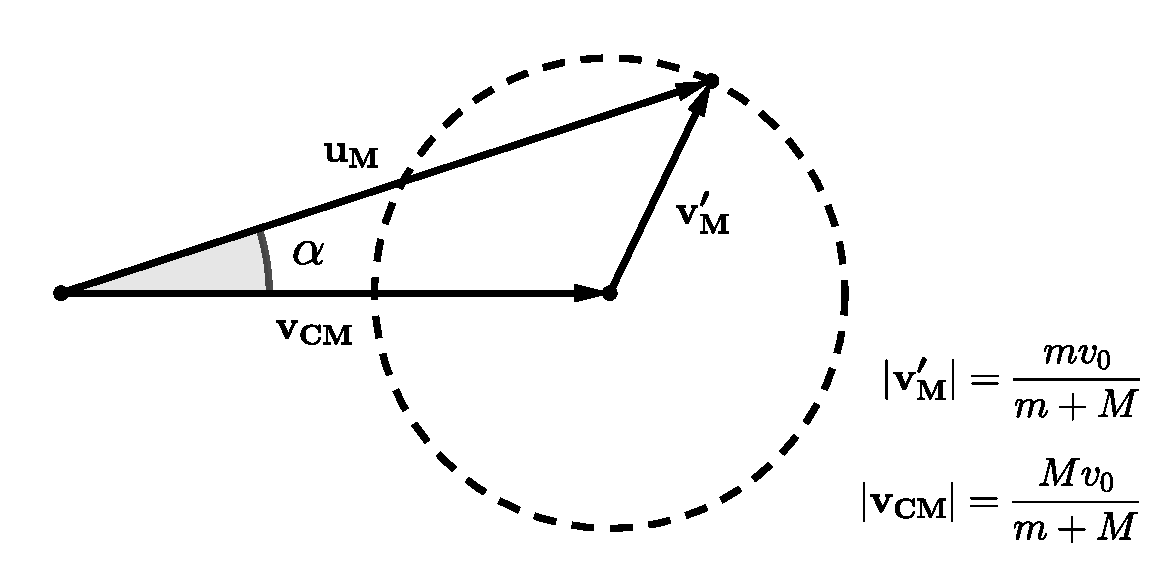
\includegraphics[width=0.6\textwidth]{fig/a2008_s3.pdf}
\end{center}

From the diagram we see that the deviation of $\mathbf{u_M}$ from $\mathbf{v_0}$ is largest when the vector $\mathbf{u_M}$ ends up tangent to the circle of $\mathbf{v_M'}$. In that case,
\begin{equation*}
\left.	\sin{\alpha}=\frac{mv_0}{m+M} \middle/ \frac{Mv_0}{m+M} = m/M \right.
.
\end{equation*}
Then $\boxed{\alpha=\arcsin{(m/M)}.}$\\

(b) When $\alpha$ is largest, the velocities are related by $|\mathbf{u_M}|^2+|\mathbf{v_M'}|^2=|\mathbf{v_{CM}}|^2$. This gives us 
\begin{equation*}
\boxed{u_M=\sqrt{\frac{M-m}{M+m}}v_0}\,
.
\end{equation*}
To find $u_m$, we will use $\mathbf{u_m}=\mathbf{v_m'}+\mathbf{v_{CM}}$. The vector $\mathbf{v_m'}$ makes an angle $\frac{\pi}{2}-\alpha$ with the $x$-axis and has the same magnitude as $\mathbf{v_{CM}}$. Using the law of cosines, we find 
\begin{equation*}
	|\mathbf{u_m}|=\sqrt{2(1+\sin\alpha)}\, |\mathbf{v_{CM}}| \quad\quad\Rightarrow\quad\quad \boxed{u_m=\sqrt{\frac{2M}{m+M}}v_0}\,.
\end{equation*}
\end{solution}
\fi

\end{document}
